% final draft
% todo: Interkapitel-Referenzen, Kontextgrafik

\chapter{Anforderungen an ein Werkzeug} % (fold)
\label{cha:anforderungen}

Dieses Kapitel dient der Überleitung von den bislang auf konzeptueller Ebene beschriebenen Überlegungen hin zur tatsächlichen Umsetzung der Werkzeugunterstützung für „Articulation Work“ mittels der Externalisierung und Abstimmung mentaler Modelle. Basierend auf den Erkenntnissen aus den Kapiteln \ref{cha:articulation_work} und \ref{cha:mentale_modelle} sowie der in Kapitel \ref{cha:methodik} entwickelten Methodik werden hier die funktionalen Anforderungen an das Werkzeug beschrieben. Abbildung \ref{fig:img_Kontextgrafiken_k5} stellt dieses Kapitel und dessen Aufbau im Kontext der anderen inhaltlich vor- und nachgelagerten Kapitel dar.


\begin{figure}[htbp]
	\centering
		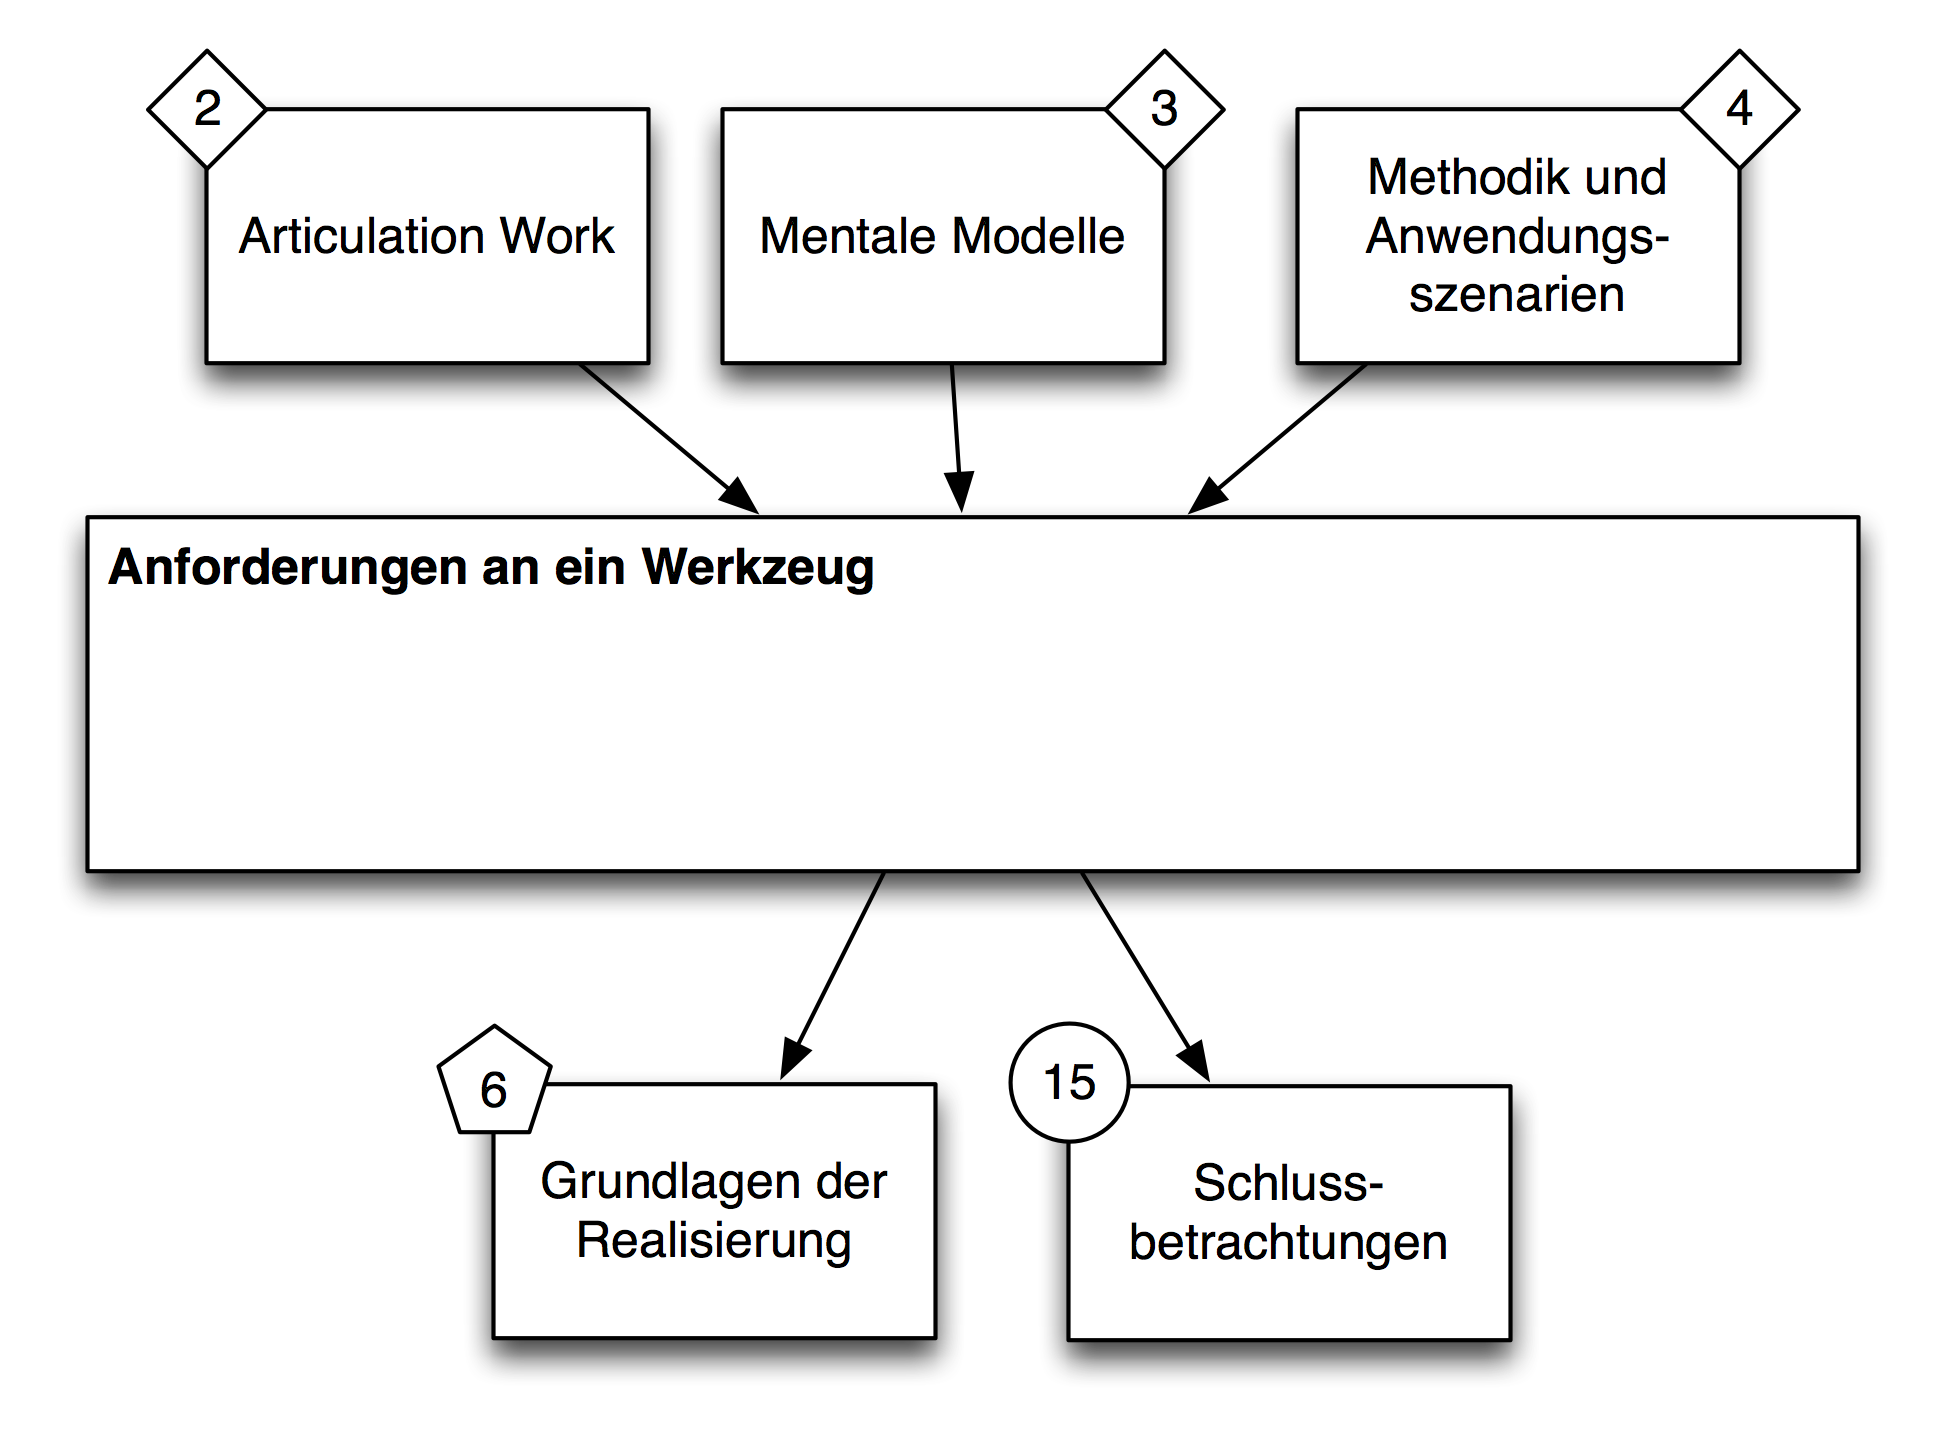
\includegraphics[scale=0.6]{img/Kontextgrafiken/k5.png}
	\caption{Kapitel „Anforderungen an ein Werkzeug“ im Gesamtzusammenhang}
	\label{fig:img_Kontextgrafiken_k5}
\end{figure}

Die Anforderungen lassen sich jeweils auf einen von drei dieser Arbeit zugrunde liegenden Ansätzen zurückführen, die in den Kapiteln \ref{cha:articulation_work} und \ref{cha:mentale_modelle} beschrieben sind. Größtenteils sind sie direkte Konsequenzen auf den Vorgaben hinsichtlich Struktur und Vorgehen, die von Strukturlegetechniken oder Concept Mapping gemacht werden. Es ist jedoch zusätzlich notwendig, auf die zur Durchführung expliziter „Articulation Work“ selbst zurückzugreifen, um die Eignung des Werkzeugs nicht nur für generische Externalisierung von mentalen Modellen selbst sicherzustellen. Vielmehr muss auch die Berücksichtigung der speziellen Anwendungsbedingungen und Betrachtungsgegenstände im Rahmen von „Articulation Work“ gewährleistet werden.

\section{Anforderungen aus Strukturlegetechniken} % (fold)
\label{sec:anforderungen_aus_strukturlegetechniken}

\begin{anf}
	\label{anf:physische_abbildung_legen_beliebiger_diagrammatischer_modelle}
	Physische Abbildung beliebiger diagrammatischer Modelle
\end{anf}
 % (fold)


Ein Werkzeug zur Unterstützung von Strukturlegetechniken muss das grundlegende Konzept der Methodik vollständig unterstützten. Es muss möglich sein, Konzepte auf einer Modellierungs-Oberfläche zu platzieren und zueinander in Beziehung zu setzen. Der gesamte Modellstatus muss visuell auf der Oberfläche erkennbar sein.

% paragraph physische_abbildung_legen_beliebiger_diagrammatischer_modelle (end)

\begin{anf}
	\label{anf:unterstützung_der_iterativen_aushandlung_des_modells}
	Unterstützung der iterativen Aushandlung des Modells
\end{anf}
 % (fold)


Im Sinne der Unterstützung der Dialog-Konsens-Methodik sind ist der Austausch über das Modell durch das Werkzeug zu unterstützen. Vor allem muss es möglich sein, Anmerkungen über Konsens oder Dissens über einzelnen Modellteile oder das gesamte Modell explizit mit in die Repräsentation aufzunehmen. 

% paragraph unterstützung_der_iterativen_aushandlung_des_modells (end)

\begin{anf}
	\label{anf:ermöglichung_experimenteller_veränderungen_am_modell}
	Ermöglichung experimenteller Veränderungen am Modell
\end{anf}
 % (fold)

Es muss möglich sein, das Modell experimentell zu verändern und ggf. zu einem früheren stabilen Modellzustand zurückzukehren. Dies erlaubt eine konsequenzlose Erkundung von Lösungsräumen und unterstützt damit den Dialog-Konsens-Prozess. Das Werkzeug muss also stabile Modellzustände erfassen und deren Rekonstruktion unterstützen.

% paragraph ermöglichung_experimenteller_veränderungen_am_modell (end)

% section anforderungen_aus_strukturlegetechniken (end)

\section{Anforderungen aus Concept Mapping} % (fold)
\label{sec:anforderungen_aus_concept_mapping}

\begin{anf}
	\label{anf:nicht_vorgegebene_semantik_der_modellierungselemente}
	Nicht vorgegebene Semantik der Modellierungselemente
\end{anf}
 % (fold)

Wie oben bereits argumentiert und auch aus \citet{Seel91}\footnote{siehe Seite \pageref{anforderungen_seel} in dieser Arbeit} abzuleiten, sind zur Unterstützung von expliziter „Articulation Work“ vor allem Varianten von Strukturlegetechniken geeignet, die im Sinne von Concept Mapping keine Vorgaben hinsichtlich der zu verwendenden Konzepte und Verknüpfungen machen. Das Werkzeug muss dementsprechend die Offenheit bieten, beliebige Klassen von Konzepten und Verknüpfungen zu definieren (z.B. Klasse „organisationale Rolle“) und von diesen beliebige Instanzen zu bilden und zu benennen (z.B. Instanz „Geschäftsführer“). Gleichzeitig muss sichergestellt werden, dass die festgelegte Semantik im Modell mit abgebildet wird und nicht verloren geht.

% paragraph nicht_vorgegebene_semantik_der_modellierungselemente (end)

\begin{anf}
	\label{anf:verknüpfung_mit_digitalen_ressourcen}
	Verknüpfung mit digitalen Ressourcen
\end{anf}
 % (fold)

Die Einbindung von digitalen Ressourcen (Dateien, Hyperlinks,\ldots) ermöglicht die Einbindung des Modells in den organisationalen Kontext und erleichtert so einerseits die Verständnisbildung und ermöglicht andererseits die Verwendung der Repräsentation als unmittelbare Handlungsanleitung mit Verknüpfungen zu den betroffenen Arbeitsgegenständen (siehe dazu auch die Beschreibung von \citep{Jorgensen04} auf Seite \pageref{steps:jorgensen} in dieser Arbeit).

% paragraph verknüpfung_mit_digitalen_ressourcen (end)

\begin{anf}
	\label{anf:bearbeitung_von_beliebig_komplexen_modellen}
	Bearbeitung von beliebig umfangreicher Modellen
\end{anf}
 % (fold)

Umfangreiche Modelle enthalten oft eine große Anzahl von Konzepten und viele Verknüpfungen. Das Werkzeug muss das Modell in einer Form darstellen, die dessen Erfassung und Manipulation ermöglicht, ohne die Repräsentierenden kognitiv zu sehr zu belasten.
% paragraph bearbeitung_von_beliebig_komplexen_modellen (end)

% section anforderungen_aus_concept_mapping (end)

\section{Anforderungen aus Articulation Work} % (fold)
\label{sec:anforderungen_aus_articulation_work}

\begin{anf}
	\label{anf:kollaborative_und_unmittelbare_manipulierbarkeit_des_modells}
	Kooperative und unmittelbare Manipulierbarkeit des Modells
\end{anf}
 % (fold)

Zur Unterstützung von expliziter „Articulation Work“ muss das Werkzeug kooperative Strukturlege-Prozesse erlauben. Es muss möglich sein, das gelegte Modell simultan zu erweitern oder zu verändern.

% paragraph kollaborative_und_unmittelbare_manipulierbarkeit_des_modells (end)

\begin{anf}
	\label{anf:persistente_ablage_des_modells_möglichkeit_zur_rekonstruktion}
	Persistente Ablage des Modells und Möglichkeit zur Rekonstruktion
\end{anf}
 % (fold)

Die persistente Ablage eines Modells (z.B. als digitale Repräsentation) und Werkzeugunterstützung zur Rekonstruktion eines abgelegten Modells erlaubt die Wiederaufnahme eines unterbrochenen Strukturlegeprozesses bzw. die Reflexion und Anpassung bereits erstellter Modelle zu einem späteren Zeitpunkt. Diese Forderung wird auch von \citet{Herrmann02} angeführt (siehe Seite \pageref{steps:herrmann} in dieser Arbeit) und unter anderem von \citet{Shipman00} zur Nachvollziehbarkeit bei Erstellung und Konsum von vernetzen Inhalten (dort: Hypertext) vorgeschlagen\footnote{\emph{„By recording and replaying the authoring process, navigable history can re-situate an author after a gap in the authoring process. Similarly, in a collaborative authoring process, an author can play through the events since his/her last authoring session to quickly determine the activity of the other authors. Finally, in many situations, information becomes harder to interpret as its context changes over time. By returning to the state of the information space at the time of authoring, disambiguation of the information may become possible. For the reader who is not also the writer of the hypertext there are additional uses of navigable history. A reader replaying the author’s writing process can gain insight into the motivation of the author and have a greater understanding of the author’s writing style. Such an understanding is important in collaborative work and in other contexts, like education and literary analysis.“} \citep{Shipman00}}.

% paragraph persistente_ablage_des_modells_möglichkeit_zur_rekonstruktion (end)

% section anforderungen_aus_articulation_work (end)

\section{Grundlegende Technologieentscheidung} % (fold)
\label{sec:grundlegende_technologieentscheidung}

Basierend auf den oben identifizierten Anforderungen kann nun eine grundlegende Entscheidung hinsichtlich der Technologie zur Umsetzung der Werkzeugunterstützung getroffen werden. Aufgrund der Anforderungen, die aus dem Bereich der „Strukturlegetechniken“ sowie „Articulation Work“ selbst abgeleitet wurden, ist die Unterstützung durch ein Werkzeug notwendig, das die Erstellung und Repräsentation der Modelle im physischen Raum ermöglicht.

Ein Teil der Anforderungen, die im Bereich des „Concept Mapping“ und ebenfalls wieder der „Articulation Work“ identifiziert werden konnten, können hingegen nur realisiert werden, wenn das Werkzeug mit rechner-unterstützter Funktionalität angereichert wird.

Einerseits ist es nun also notwendig, das Modell physisch abzubilden, was der Verwendung eines Werkzeugs mit  bildschirmbasierter Benutzungsschnittstelle entgegensteht. Andererseits ist zur Umsetzung mancher Anforderungen die Verwendung eines Rechners notwendig, so dass das Modell auch digital erfasst und repräsentiert werden muss.

Ein Ansatz der Mensch-Maschine-Interaktion, der die Verwendung von interaktiven Systemen mit nicht-traditionellen Benutzungsschnittstellen untersucht, ist jener der \emph{„Tangible Interfaces“}. Als „Tangible Interfaces“ werden im Allgemeinen Benutzungsschnittstellen bezeichnet, die ein Computersystem mit auf den jeweiligen Anwendungsfall abgestimmten physischen Artefakten kontrollierbar machen, die gleichzeitig zur Informationsausgabe durch das Computersystem verwendet werden.

Für den hier vorliegenden Anwendungsfall -- der interaktiven kooperativen Erstellung von diagrammatischen Modellen -- bietet sich die Verwendung eines \emph{„Tangible Tabletop Interface“} an. Als Spezialfall eines „Tangible Interface“ wird hier eine Tischoberfläche als Ein- und Ausgabekanal verwendet, auf dem physische Artefakte zur Interaktion mit dem System verwendet werden. Die Ähnlichkeit dieses Ansatzes mit dem Anwendungsszenario im Falle von „Strukturlegetechniken“ spricht für eine Verwendung von „Tangible Tabletop Interfaces“ zur Umsetzung des in dieser Arbeit zu entwickelnden Werkzeugs. 

% section grundlegende_technologieentscheidung (end)

\section{Zusammenfassung}
\label{sec:anforderungen_zusammenfassung}

In diesem Kapitel wurden die Anforderungen an das zu entwickelnden Werkzeug aus den Ergebnissen der Kapitel \ref{cha:articulation_work}, \ref{cha:mentale_modelle} und \ref{cha:methodik} abgeleitet. Insgesamt konnten \theanf \ Anforderungen identifiziert werden, die hier -- unabhängig von der konkreten Umsetzung -- rein aus Sicht der konzeptuell zu unterstützenden Tätigkeit beschrieben wurden.

Im letzten Abschnitt dieses Kapitels wurde auf Basis der Ergebnisse der Anforderungserhebung jene Klasse von Systemen identifiziert, deren Verwendung die grundlegende Forderung nach physischer Modellbildung und gleichzeitiger Unterstützung durch computerbasierte Werkzeuge erfüllen kann. „Tangible Interfaces“ sind hier mit ihrem Anspruch, konkrete, physische Benutzungsschnittstellen für interaktive Computersysteme zur Verfügung zu stellen, durch die Ähnlichkeiten zu „Strukturlegetechniken“ bei der gleichzeitigen Möglichkeit zur Umsetzung von rechnergestützten Funktionen einsetzbar.

\subsection{Beitrag zur globalen Zielsetzung}

Die in diesem Kapitel formulierten Anforderungen bilden die Brücke zwischen Methodik und Werkzeug im Rahmen der Beantwortung der in Kapitel \ref{cha:einführung} formulierten Fragestellung \ref{tf:technik} („Wie kann ein Instrument zur Unterstützung von expliziter Articulation Work umgesetzt werden?“).

Am Ende von Teil \ref{prt:grundlagen} beschriebene Methodik ist Teil des zur Unterstützung von „Articulation Work“ konzipierten Instruments. Dieses wird durch das durch die hier formulierten Anforderungen hinsichtlich seiner Funktionalität festgelegten Werkzeug zu jene Instrument ergänzt, das Gegenstand der Fragestellung \ref{tf:technik} ist.

Die hier formulierten Anforderungen repräsentieren gleichzeitig die aus methodischer Sicht notwendigen Funktionen zur Unterstützung des kooperativen Externalisierungs- und Abstimmungsprozesses und damit der Durchführung von „Articulation Work“ ab. Die Erfüllung der Anforderungen ist damit eine Voraussetzung zur effektiven Unterstützung von  „Articulation Work“. In diesem Sinne sind sie auch ein Beitrag zur Beantwortung der Fragestellung \ref{tf:beurteilung_der_effektivität} („Wie kann die Effektivität der Unterstützung von expliziter Articulation Work beurteilt werden?“) und müssen als Beurteilungskriterien herangezogen werden.

\subsection{Weitere Verwendung der Ergebnisse}

In den folgenden Kapiteln wird nun aufbauend auf der Grundsatzentscheidung für die Entwicklung eines „Tangible Interfaces“ das Werkzeug in allen in den Anforderungen angesprochenen Aspekten spezifiziert. Zusätzlich sind auch jeweils die konkrete technische Umsetzung sowie allfällige Einschränkungen, die diese Umsetzung mit sich brachte, beschrieben.

Kapitel \ref{cha:implementierung_Überblick} geht -- noch unabhängig von dem konkreten hier entwickelten Werkzeug -- auf die Eigenschaften von Tangible Interfaces und deren Spezifikation ein. Daneben wird in diesem Kapitel auch die „Related Qork“ aus konzeptueller und technischer Sicht aufgearbeitet. In den Kapiteln \ref{cha:input_&_interpretation}, \ref{cha:visualisierung} und \ref{cha:persistierung} werden die Implementierungsalternativen und die konkrete Umsetzung des Werkzeugs getrennt für die Eingabe von Information (also die Modellbildung selbst), die Ausgabe von Information sowie die Sicherstellung der Persistierung der Modelle beschrieben. Die Überprüfung der Erfüllung der hier spezifizierten Anforderungen ist Gegenstand der Kapitel \ref{cha:eval_werkzeug} und \ref{cha:eval_modell}, die Teil der Beschreibung der Evaluierung des hier entwickelten Systems sind.

% chapter anforderungen (end)